\documentclass{article}

%\usepackage[
  paperheight=8.5in,
  paperwidth=5.5in,
  left=10mm,
  right=10mm,
  top=20mm,
  bottom=20mm]{geometry}
\usepackage[utf8]{inputenc}

%%\usepackage{biblatex}
\usepackage{graphicx}
\usepackage{wrapfig}
\usepackage[bottom]{footmisc}
\usepackage{listings}
\usepackage{enumitem}

\usepackage{wrapfig}
\usepackage{ragged2e}

\usepackage{array}
\usepackage[table]{xcolor}
\usepackage{multirow}
\usepackage{booktabs}
\usepackage{hhline}
\definecolor{palegreen}{rgb}{0.6,0.98,0.6}

\usepackage{amsmath}
\usepackage{amssymb}
\usepackage{multicol}
\usepackage{lipsum}
\usepackage{hyphenat}
\PassOptionsToPackage{hyphens}{url}
\usepackage{url}

\usepackage{rotating}

\usepackage{pdfpages}

%% support use of straight quotes in code listings
\usepackage[T1]{fontenc}
\usepackage{textcomp}
\usepackage{listings}
\lstset{upquote=true}

%% for shrinking space between lines
\usepackage{setspace}

\usepackage{caption}

\newcommand*{\affaddr}[1]{#1} % No op here. Customize it for different styles.
\newcommand*{\affmark}[1][*]{\textsuperscript{#1}}
\newcommand*{\email}[1]{\small{\texttt{#1}}}
\newcommand{\tarot}{\textsc{Tarot}}
\renewcommand*\contentsname{\centering Table of Contents}

\renewcommand{\footnoterule}{%
  \kern -3pt
  \hrule width \textwidth height 0.5pt
  \kern 2pt
}

\usepackage{titlesec}
\titleformat*{\section}{\large\bfseries}
\titleformat*{\subsection}{\normalize\bfseries}
\titleformat*{\subsubsection}{\normalize\bfseries}

% define variables
\newcommand{\confOrdinal}{34th}
\newcommand{\confName}{South Central}
\newcommand{\confDates}{March 31st}
\newcommand{\confYear}{2023}
\newcommand{\confSchool}{Stephen F. Austin State University}
\newcommand{\confCity}{Nacogdoches, TX}
\newcommand{\journalVolume}{38}
\newcommand{\journalNumber}{7}
\newcommand{\journalMonth}{April}
\newcommand{\journalYear}{2023}
\newcommand{\regionalEditor}{Mustafa Al-Lail}
\newcommand{\regionalEditorSchool}{Texas A\&M International University}



%%\addbibresource{sample.bib}

\title{Preparing ABET Accreditation for An Undergraduate Software Engineering Program\footnote{\protectCopyright \copyright \confYear\ by the Consortium for Computing Sciences in Colleges.
Permission to copy without fee all or part of this material is granted provided
that the copies are not made or distributed for direct commercial advantage,
the CCSC copyright notice and the title of the publication and its date appear,
and notice is given that copying is by permission of the Consortium for
Computing Sciences in Colleges.  To copy otherwise, or to republish, requires
a fee and/or specific permission.
}
}

\author{
Jicheng Fu, Myungah Park, Gang Qian,\\
Hong Sung, Thomas Turner\\
Department of Computer Science\\
University of Central Oklahoma\\
Edmond, OK 73034\\
\email{gqian@uco.edu}
}

\begin{document}
\maketitle

\begin{abstract}
In this article, we share our seven-year experience in preparing for ABET accreditation for the undergraduate Software Engineering program offered at the University of Central Oklahoma.  We present our approach to the preparation with a focused discussion of the general and the program-specific accreditation criteria required by ABET Engineering Accreditation Commission.  As most computer science graduates work in the area of software development, we hope our experience can benefit computer science departments similar to our setup and promote better undergraduate education in the area of software engineering.
\end{abstract}

\section{Introduction}
The BS in Software Engineering (SE) program was created at the University of Central Oklahoma (UCO) in 2014.  Before that, the department had been offering a BS in Computer Science program for almost thirty years.  Our motivation to create the SE program was multifold.  First, while SE used to be considered as a sub-discipline of Computer Science (CS), software systems had grown larger, more complex, and more expensive, some of which were even mission critical.  As a result, SE was eventually recognized as a discipline of its own by many professionals in the IT industry.  Second, it was our observation that most of our CS graduates worked in positions related to software design and development.  Based on feedback from our alumni and the department’s industrial advisory board, offering a program that focused on the lifecycle of software systems would greatly benefit our graduates for their career in the software industry. 

After the BS in SE program was created, an immediate next step for us was to prepare for ABET accreditation.  The department received ABET accreditation for its CS major in 2007, of which we recognized the benefits as follows: 1) it increased the recognition of the program from the university administration; 2) it increased the recognition of the program from its external stakeholders, especially prospective students; and 3) it helped maintain an objective academic standard that was established by third-party experts in the CS discipline.  Our experience of having the CS major accredited was documented in \cite{gourley08} and \cite{fu14}.

To accredit the new SE program, we worked with a different ABET Commission.  While all computing disciplines are reviewed and accredited by ABET Computing Accreditation Commission (CAC), all engineering programs are evaluated by ABET Engineering Accreditation Commission (EAC).  Therefore, we studied and implemented ABET standards for engineering programs before the ABET EAC review of 2019.  The remainder of the paper discusses the details of our approach to preparing for ABET accreditation with a focus on both the general and the SE program-specific accreditation criteria.  

\section{Preparing for the ABET Evaluation}
Our preparation for the ABET evaluation of our SE program included the following features:
\begin{enumerate}[noitemsep]
  \item Having an existing program accredited by ABET
  \item Having a member of the faculty serve as an ABET volunteer
  \item Performing a dress rehearsal for the SE program accreditation visit
\end{enumerate}

While none of features above were mandatory, each of them provided support in the accreditation process.  Having an existing program accredited by ABET meant that the department had a working infrastructure for documentation to support ABET accreditation.  As indicated by Leach \cite{leach10}, documentation is important; if it is not written, it does not exist. The department had a process for establishing and reviewing program educational objectives (see Section \ref{peo}).  We also had functioning assessment tools and procedures to enable continuous improvement.  A method for collecting required documents for courses and storing them electronically was instituted too. The sum of these activities served as a foundation for accrediting the SE program.  
        
Having a member of the department serve as an ABET volunteer provided detailed insights as to how ABET accreditation was performed: this knowledge was invaluable in preparing for ABET visits.  The institution and the department recognized the effort of the ABET volunteer, demonstrating support for the ABET accreditation process as recommended by Collofello \cite{collofello04}.
        
Based on prior experiences, the department believed that a dress rehearsal for a future ABET evaluation would be best.  We contacted the ABET Foundation, now called the ABET Bridge, and asked for a former team chair whose area of expertise was in the area of SE.  The ABET Foundation found a consultant having the appropriate credentials, who reviewed a self-study that we prepared and visited our institution to conduct a review exactly as an ABET team would do.  Based on the consultant’s observations, we revised the assessment processes and the materials taught in some classes to conform to the consultant’s suggestions.  

\section{ABET Criteria for Software Engineering Programs}
In this section, we present in detail how we met the ABET criteria for Software Engineering programs, which must be followed by every accredited SE program.   As mentioned earlier, ABET EAC accredits Software Engineering programs instead of ABET CAC.  The 2022-23 Criteria can be found at \cite{abet22}. The Criteria are divided into the General Criteria for Baccalaureate Level Programs, General Criteria for Master’s Level and Integrated Baccalaureate – Master’s Level Engineering Programs, and Program Criteria.  In this paper, we limit our discussion to the baccalaureate-level General Criteria as well as the Program Criteria for SE programs.  ABET evaluates programs to ensure that they satisfy both the General and the Program Criteria.
        
There are eight General Criteria and two Program Criteria for SE programs.  The Criteria are discussed in each of the following subsections.  The two SE Program Criteria are related to curriculum and faculty so they are discussed in the related General Criteria subsections (sections \ref{cur} and \ref{fac}, respectively).

\subsection{Criterion 1. Students}
Criterion 1 is about student admission, performance evaluation, transfers, advisement, and graduation requirements. This criterion ensures that students are advised regarding curriculum and career matters, attain all outcomes by the time of graduation, are awarded appropriate academic credits for all courses, and satisfy all graduation requirements.

As mentioned in the previous paragraph, student advisement is a major concern of this criterion. When we obtained ABET accreditation for our CS major, the faculty advised every student every semester.  The workload became unsustainable as our enrollment more than doubled in the past ten years.  As a result, we reformed our advisement process.  Each semester, we only offer advisement to new students to the department (transfers, major changes, and freshmen) as well as those who try to enroll into a few key courses in the curriculum, including Programming II, Data Structures \& Algorithms, and the SE Senior Design.  We used a combination of enrollment holds and instructor permissions to enforce the mandatory advisement process.  Each advisement session was documented.  This approach reduced our workload by half.   

We complied with the admission requirements set forth by the university to accept new students and transfer students. There were no additional admission requirements for students who chose to pursue the SE degree. Student performance was evaluated based on the student outcomes that ABET specifies in Criterion 3 (see Section \ref{3.3}). It was the department’s responsibility to create and administer assessment instruments to evaluate student outcomes.

Another concern of this criterion was awarding credits to transfer students.  In this case, we handled the SE program in the same way as we handled our ABET-accredited CS major.  In general, we required that all upper-division SE and CS courses be taken at UCO.  The details can be found in \cite{fu14}. 

\subsection{Criterion 2. Program Educational Objectives} \label{peo}
ABET EAC shares the same definition of Program Educational Objectives (PEOs) as that of ABET CAC, which are ``... broad statements that describe what graduates are expected to attain within a few years after graduation''.  It is important to note that the specified attainments in the PEOs should not be acquirable by a student before his/her graduation.  The PEOs should only be obtained after the student graduates.  

Criterion 2 requires that PEOs be consistent with the mission of the institution.  In addition, a review process of the PEOs, which involves constituencies of the program, must be conducted and documented with a regular cycle \cite{fu14}.  We ensured that every PEO was directly supported by one or more student outcomes (see Section \ref{3.3}) to satisfy General Criterion 3.  The department published the PEOs on the department website as required by ABET.

\subsection{Criterion 3. Student Outcomes} \label{3.3}
Student Outcomes (SOs) describe ``what students are expected to know and be able to do by the time of graduation''. There are seven ABET-defined SOs under Criterion 3, which describe the knowledge, skills, and behaviors that students should acquire through the program.  We directly adopted all seven ABET SOs as the SOs of the SE program.  Note that SOs must be periodically reviewed, and a program can choose to define its own SOs \cite{fu14}. 

Every SO needs to be related to its corresponding PEOs.  In our self-study report for accreditation, we utilized a table format to illustrate how each PEO was supported by the SOs.  For example, as shown in Table \ref{so_peo}, PEO (b) was supported by SOs \#3, \#4, \#5, \#6, and \#7.

\begin{table}[ht]
\caption{Mapping of SOs to PEOs} 
\label{so_peo} 
\centering % used for centering table
\begin{tabular}{c c c c c c c c} % centered columns (4 columns)
\hline\hline %inserts double horizontal lines
PEOs  &  \multicolumn{7}{c}{SOs}\\
\hline % inserts single horizontal line
& \#1 & \#2 & \#3 & \#4 & \#5 & \#6 & \#7 \\ [0.5ex] % inserts table
%heading

(a) & x & x & x & x & x & x & x \\ 
(b) &   &   & x & x & x & x & x \\
(c) & x &   &   &   &   & x & x \\ %[1ex] % [1ex] adds vertical space
\hline %inserts single line
\end{tabular}
\end{table}

\subsection{Criterion 4. Continuous Improvement}
Criterion 4 requires that students must be assessed to evaluate the extent to which SOs are being attained on a regular basis.  ABET defines Assessment as ``one or more processes that identify, collect, and prepare data to evaluate the attainment of student outcomes''.  It defines Evaluation as ``one or more processes for interpreting the data and evidence accumulated through assessment processes''.

Criterion 4 was the most time consuming and difficult criterion for us to satisfy.  As a first step, we needed to establish the assessment instruments.  For our ABET-accredited CS major, we used to rely on a locally defined test as the main instrument \cite{fu14}.  This approach worked for ABET accreditation purposes.  However, we found that it was difficult for us to fully utilize the assessment/evaluation results for continuous improvement.  Therefore, we decided to switch to a course-oriented approach.  

For each SO, we started by identifying all the courses where students were being prepared to attain that SO.  Among the courses identified, we picked one course that was a required course for the SE program, in which the specific SO would be assessed.  The next step was to choose one or more performance criteria (PCs) to evaluate the SO.  The number of PCs to use can be determined based on the complexity of the SO.  For simple SOs, a single PC is sufficient.  For complex ones, two or even more PCs may be needed.  For example, for SO\#6, ``an ability to develop and conduct appropriate experimentation, analyze and interpret data, and use engineering judgment to draw conclusions'', we defined two PCs as follows:

\begin{itemize}[noitemsep]
\item PC\#1 for SO\#6: An ability to development and conduct appropriate experimentation
\item PC\#2 for SO\#6: An ability to analyze and interpret data, and use engineering judgment to draw conclusions
\end{itemize}

Once the PCs are settled for an SO, artifacts produced by students in the chosen course should be used as the assessment instrument for each PC.  Note that ABET requires direct measures be used in this process.  Therefore, we needed to use actual work produced by students (indirect measures such as opinion surveys would not count).  Depending on the nature of the PC, a homework assignment, a course project, or a test can be used from the chosen course.  Note that an assessment instrument need not to be the entire assignment or test.  A part of an assignment or test can also serve as an assessment instrument.  For each artifact gathered, we defined a rubric to evaluate the artifact.  For example, an artifact might be rated in one of the following categories: Unsatisfactory, Developing, Satisfactory, or Excellent.

Figure \ref{items} provides an illustration of all the assessment items discussed above.  As shown in the figure, the course SE 4213 was chosen for the assessment of SO\#2.  SO\#2 had two PCs.  PC\#1 used the course project as its assessment instrument while PC\#2 used the second test of the course as its assessment instrument.

\begin{figure}[htbp]
\centering
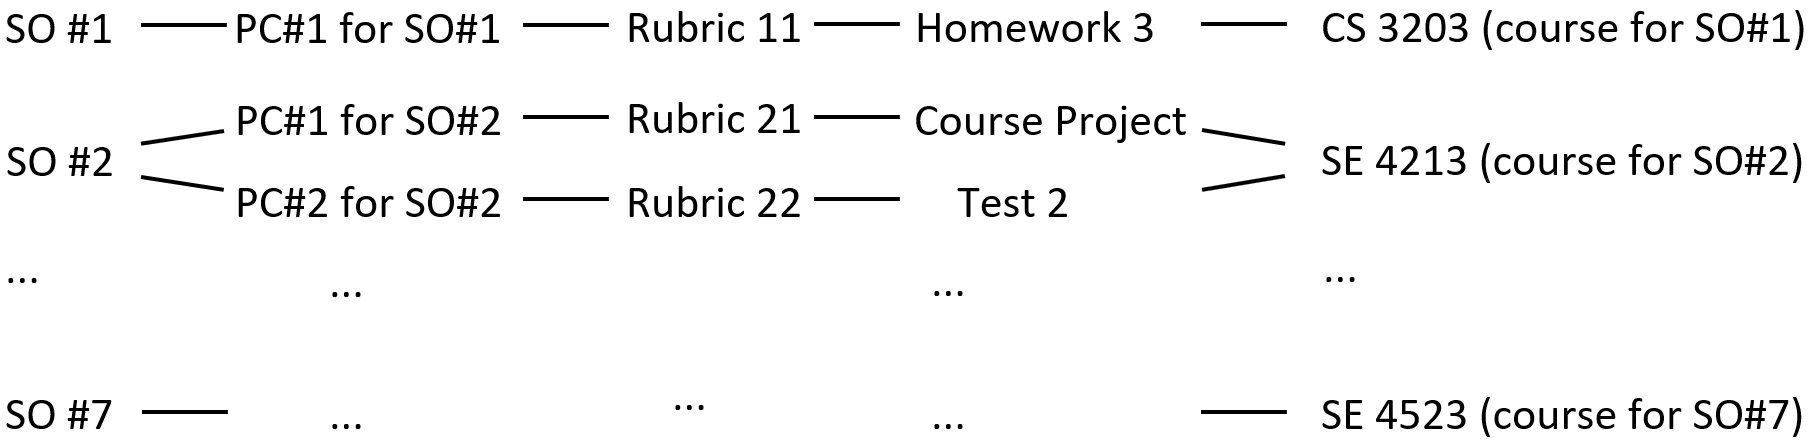
\includegraphics[width=\textwidth]{449_1.png}
\caption{Illustration of Relationships of the Assessment Items}
\label{items}
\end{figure}

After the course-oriented assessment structure was established, we set up an evaluation schedule since ABET requires continuous assessment cycles.  In the schedule, artifacts gathered in the spring and fall semesters of the prior calendar year were evaluated in the spring of the subsequent calendar year.  For example, artifacts gathered in the spring and fall semesters of 2018 were evaluated in the spring of 2019.  Annual assessment reports were produced to document the results of evaluating all SOs.  In the annual assessment reports, we identified opportunities for improving the SE program. The department’s assessment committee decided upon which of these opportunities the department would act, based on resources available and the effort required to address the opportunity.

\subsection{Criterion 5. Curriculum} \label{cur}
We must meet both the General Criterion and the SE Program Criterion on Curriculum as set by ABET.  The General Criterion specifies the subject area and the number of credit hours required for mathematics, basic science, and engineering topics without naming specific courses.  The Program Criterion mandates SE-related topics such as computing fundamentals, discrete math, software design and construction, requirements analysis, security, and software verification and validation.  

We ensured that every required SE topic was covered and every SO was supported by some course(s) in the curriculum.  As mentioned earlier, the department offered the SE program along with an ABET-accredited CS major. Many of the courses were shared between the two degrees. Several lower-division courses were characterized to meet both the CS and the SE curricula for ABET accreditation.  

At the upper-division level, three dedicated SE courses were created along with a capstone course for senior design.  The program offered three application areas, including application development, system development, and a newly added cybersecurity track.  Students in the SE program could take CS courses as electives based on the application area that they chose. 

This criterion also requires that course collectible items be kept for each time a course is taught.  In addition, a program needs at least one graduate under an ABET-compliant curriculum to qualify for an onsite visitation for accreditation \cite{fu14}.  

\subsection{Criterion 6. Faculty} \label{fac}
General Criterion 6 covers faculty size, expertise and experience while the SE Program Criterion on Faculty requires that the core SE faculty members maintain currency in their areas of professional or scholarly specialization.  At the time when we applied for ABET accreditation, there were nine full-time faculty members in the department.  Among them, seven held a Ph.D. and two held an MS degree. Most of the faculty members had also worked in the industry on software development.

ABET requires that ``collectively, the faculty must have the breadth and depth to cover all curricular areas of the program.''  To meet this requirement, two core faculty members were primarily responsible for teaching SE-related courses while other faculty members taught the rest of the required and elective courses.

Similar to the situation of many other regional universities that focused on teaching excellence, the most challenging requirement of this criterion for our department was to demonstrate that the faculty members had ongoing professional development to maintain currency.  Fortunately, we were able to adopt the same approach that we used for the accreditation of our CS major.  The actual approach was discussed in \cite{fu14}.

\subsection{Criterion 7. Facilities }
Criterion 7 examines the resources that are available to the program, such as equipment, classrooms, and laboratories.  For this criterion, we ensured that all lab computers were upgraded on a fixed five-year cycle.  Three faculty members served as system administrators for the department’s computer servers to promptly resolve any issues that might affect students’ course works. 

\subsection{Criterion 8. Institutional Support}
Criterion 8 emphasizes the importance of institutional support and leadership that must be ``adequate to ensure the quality and continuity of the program''.  Our accreditation effort was well supported by the administration at both the university and the college levels.  In general, administration support is indispensable for a program to obtain ABET accreditation.  

Our two ABET-accredited programs (SE and CS) shared the same approaches to satisfy criteria 7 and 8.  To avoid repeating ourselves, we refer our readers to \cite{fu14} for more details.

\section{Conclusion}
In this article, we presented our experience in preparing for ABET accreditation for our undergraduate SE program.  A timeline of the major events is presented as follows:
\begin{enumerate}[noitemsep]
\item Fall 2014: 		The BS in SE program was created.
\item Spring 2016: 	The first graduate of the program received his degree.  
\item Summer 2016: 	An ABET consultant visited us and provided his evaluation and feedback.  
\item Fall 2019: 		A team of ABET evaluators conducted onsite visitation.  
\item Summer 2020: 	The program was officially accredited by ABET EAC.  
\end{enumerate}

Currently, we have about 260 students in the ABET-accredited CS major and about 70 students in the SE program.  We have observed a noticeable enrollment increase in the SE program after its ABET accreditation.  The accreditation of the SE program has also led to its top national rankings by two separate online resources for prospective college students (study.com and HQUniversity).  For the next step, we will be working on ways to encourage even more students into the SE program as it provides targeted learning on software design and development, which is a much-needed skill for the professional career of most of our graduates in the industry.  

\medskip

\bibliographystyle{plain}
\bibliography{449}

\end{document}
